%-------------------------------------------------------------------------
\documentclass[authoryear,preprint,review,12pt]{elsarticle}



\setlength{\parskip}{1em}			% espaciar parrafos
\newtheorem{proposition}{Proposition}
\newtheorem{definition}{Definition}
\newtheorem{proof}{Proof}
\newtheorem{corollary}{Corollary}

\usepackage{hyperref}				% enlaces en el pdf
\hypersetup{colorlinks=true}	% colores en vez de cajas en los enlaces
\usepackage{times}              		% la letra
\usepackage{graphicx}           		% para manejar imagenes
\usepackage{subfigure}          		% para manejar subfiguras
\usepackage{tabularx}		   		% para ajustar el ancho de las columnas
%\usepackage[margin=2.5cm]{geometry}	% Change margins
\usepackage[table]{xcolor}			% Colores en el cronograma
\usepackage{multirow}				% Cabecera del cronograma
\usepackage{watermark}				% Para la portada
\usepackage{datetime}				% Fecha de creado
\usepackage{stackengine}				% Para listar los articulos en el nodo de la taxonomía
\usepackage{algorithm}				% Para el seudocódigo
\usepackage{setspace}				% Para el seudocódigo
\usepackage{amsmath}					% Para el seudocódigo
\usepackage[noend]{algpseudocode}	% Para el seudocódigo
\usepackage{multicol}				% Para el seudocódigo
%\usepackage{algorithmic}

\begin{document}
	
	\title{A New Algorithm for Reduct Computation Based on the Pruning Properties of Gap Elimination 
		   and Attribute Contribution}
		
	
	\address{Computer Science Department\\National Institute of
	Astrophysics, Optics and Electronics\\
	Luis Enrique Erro \# 1, Santa Mar\'{\i}a Tonantzintla, Puebla,
	72840, M\'{e}xico} 
	
	\begin{abstract}
		Attribute reduction is a key aspect of Rough Set Theory.  Finding the complete set of reducts is relevant 
		in several real-world applications such as the assessment of attribute relevance, multi--objective 
		cost--sensitive attribute reduction and dynamic reduct computation. The main limitation in the application
		of Rough Set methods is that finding all reducts of an information system has exponential complexity 
		regarding its number of attributes. Several algorithms have been reported to reduce the execution time
		of reduct computation. Unfortunately, most of these algorithms relay on complex operations and data
		structures. Therefore, in this paper we propose a new algorithm for computing all the reducts of an
		information system, based on binary cumulative operations, which uses the properties of Gap 
		elimination and Attribute Contribution for pruning the search space. Finally, the proposed algorithm is
		evaluated over synthetic and standard datasets.
	\end{abstract}
	
	\begin{keyword}
		Rough Sets\sep Reduct Computation\sep Typical Testor.
	\end{keyword}

	\maketitle

%-------------------------------------------------------------------------------
% your earth-shattering contribution

\section{Introduction}
% BAsico sobre los reductos
  Rough set theory (RST), proposed by Z. Pawlak in 1981 \citep{Pawlak81,Pawlak81-2,Pawlak82,Pawlak91}, 
  is a relatively new mathematical theory to deal with imperfect knowledge, in particular with vague 
  concepts. Into RST, information systems are tables of objects (rows) described by a set of attributes (columns). 
  When data is collected or recorded, every single aspect (attribute) of the object under study is considered 
  to have a complete representation and to ensure that no potentially useful information is lost.
  As a result, information systems are usually characterized by a large number of attributes,
  however, this degrades the performance of machine learning tools \citep{Parthalain08}.
  One of the main concepts in RST is the notion of reduct, which is a minimal subset of attributes 
  preserving the discernibility capacity of the whole set of attributes \citep{Pawlak91}.  
  However, the main restriction in practical applications of RST is that computing all the reducts of an 
  information system is NP--hard \citep{Skowron92}. 
  
  Most of the work on reduct computation has been devoted to finding a single optimal reduct (having the minimum 
  number of attributes) or a reduced number of reducts. Several heuristic approaches search for a pseudo optimal
  reduct using a determined measure \citep{Zheng14,Liang2014}. Some stochastic approaches including Genetic
  Algorithms \citep{Feng2012,Hedar2015}, Ant Colony Optimization \citep{Jensen03,Chebrolu2015} and Particle Swarm 
  Optimization \citep{Chen15,Luan2015} have been also reported in order to achieve a better global optimization. 
  In this paper, on the other hand, we are focused on solving the problem of computing all the reducts of an
  information system.
  Early algorithms for computing the complete set of reducts \citep{Bazan2001,Ohrn00} are integrated in RSES and
  ROSETTA software for rough sets computation. These algorithms are unable to solve even middle size problems
  \citep{Lazo15}. The divide and conquer approach presented by \cite{Starzyk99,Starzyk00}, and then modified in
  \citep{Jensen14}, operates over the binary discernibility function, which leads to inefficient data 
  representations. Then, a faster algorithm based on several properties for pruning the search space is proposed
  by \cite{WangP07}. This is a very elaborated algorithm, its main drawback is that it works directly
  over the dataset instead of the discernibility matrix. 
  
     	
% Relación con los testores
  RST reducts have been related to the typical testors (TT) from the logical combinatorial approach 
  to pattern recognition \citep{Chikalov2013}. Testor Theory was originally created by \cite{Cheguis55} as a tool
  for analysis of problems connected with control and diagnosis of faults in circuits. 
  However, Testor Theory has been extended in order to be used for feature selection as shown in \citep{Ruiz08}
  and \citep{Martinez01}. Algorithms for typical testors computation can be applied to reduct computation due to the similarity between these two concepts \citep{Lazo15}. There have been developed two kinds of algorithms for
  computing typical testors: \emph{internal scale} algorithms, such as CT \citep{Bravo83}, CC \citep{Aguila84} 
  and YYC \citep{Alba14}; and \emph{external scale} algorithms, such as BT and TB \citep{Ruiz85}, LEX
  \citep{Santiesteban03}, CT\_EXT \citep{Sanchez07} and BR \citep{Lias09}. The former analyse the discernibility
  matrix to find out some conditions to guarantee that a subset of attributes is a typical testor. The latter
  search for typical testors over the power set of attributes, avoiding unnecessary evaluations by pruning
  some attribute subsets. Internal scale algorithms usually evaluate less candidates than external scale
  algorithms but each candidate evaluation has a higher computational cost. Therefore, the search of fast 
  algorithms for computing typical testors has been biased to external scale algorithms \citep{Alba14}.
    
% Utilidad de todos los reductos
  Although most algorithms for reduct computation search for a single reduct or a small subset of reducts, 
  the complete set of reducts of an information system is useful in some recent applications. \cite{Xu2013}
  developed a multi-objective cost-sensitive attribute reduction. First, they compute all reducts of an 
  information system. Then, they separately calculate the cost, in terms of time and money, of every reduct. 
  Finally, the worst reducts are dismissed, leaving a Pareto optimal solution set. From this smaller set of 
  reducts, a user can easily select an optimum subset. On the other hand, \cite{Mukamakuza2014} developed 
  three new algorithms for dynamic reduct computation. 
  The first step in their three algorithms is the finding of all the reducts. Then, the complete set of reducts 
  is filtered in order to obtain an optimum subset, from which dynamic reducts are computed. They showed that 
  this procedure improves the performance of dynamic reduct computation algorithms.	
  From Testor Theory, \cite{Torres2014} used the informational weight, computed through typical testors 
  (reducts), to identify risk factors on transfusion related acute lung injury; and to establish an assessment
  for each variable.  In \citep{Torres2014}, the informational weight is a percentage value, which accounts 
  for the presence of each variable (attribute) in the whole set of typical testors. These are real life
  applications for algorithms that compute the complete set of reducts or typical testors.	
	
% Relación con otros problemas de grafos
  Recently, \cite{chen2015} exposed the relation between reduct computation and the minimum vertex cover
  problem in graph theory. Given that both of these problems can be translated into the calculation of
  prime implicants of a Boolean function, they applied algorithms designed for reduct computation in the
  solution of the minimum vertex cover problem. This unification opens a new spectrum of real-world applications
  for fast reduct computation algorithms. They stood that the vertex cover problem has been used in applications 
  such as crew scheduling, VLSI design, nurse scheduling and industrial machine assignments.
  The connexion with the problem of computing the prime implicants of a Boolean function, makes fast 
  algorithms for computing all reducts relevant in other applications. For instance, \cite{Li2015} presented
  a new technique for mining frequent patterns from the minimal disjunctive normal form.

% descripción de la propuesta
%  Latest algorithms from Testor Theory are based on fast binary cumulative operations \linebreak
%  \citep{Sanchez10,Lias13}.
  In this work, we show the advantages of fast binary cumulative operations \citep{Sanchez10,Lias13} over other 
  approaches from rough set theory \citep{WangP07,Jensen14}. Following this idea, we propose a new algorithm tackling the inefficient behavior of CT\_EXT in some cases \citep{Alba14}, by using the pruning property of gap elimination. In relation to fast-BR, which is one of the latest and fastest reported algorithms; our proposed algorithm evaluates more candidates in most cases, but the evaluation cost is lower, as it will be shown in our experiments. Then we show that our algorithm performs faster than all other recent reported alternatives in
  many cases. 
  The main contribution of this work is the design and evaluation of a new algorithm for reduct computation,
  based on  the pruning properties of gap elimination and attribute contribution. In order to evaluate our proposal, experiments are carried out over several standard datasets \citep{Bache13} and synthetic data.
  
  The rest of this paper is structured as follows. Section~\ref{basicConcepts} introduces the fundamentals of
  rough set theory, particularly for decision systems; and those properties used by algorithms for the pruning
  process. 
  In Section~\ref{relatedWork}, we discuss the related work on reduct and typical 
  testors computation.  In Section~\ref{GCSBDM}, we introduce the GCSBDM algorithm for computing all reducts of an
  information system. An evaluation of the proposed algorithm and a discussion of the experimental results are 
  presented in section~\ref{evaluation}. Finally, section~\ref{conclusions} shows our conclusions and some
  directions for future work.
   
\section{Basic Concepts}\label{basicConcepts}
  RST is based on the assumption that every object an the universe of discourse is described, through a 
  set of attributes, by some information associated to it. This information constitutes the basis for the
  classification of unseen objects. RST motto is \textit{Let the data speak for themselves} \citep{Tiwari14}.
  
  From the RST point of view, two objects are indistinguishable (indiscernible) if they have an equivalent 
  value for each attribute in their description. Indiscernibility relations arising this way constitute the
  mathematical foundations of RST. 
  Some basic concepts of RST are presented bellow.
  
\subsection{Information System}
  The basic representation of data in RST is an \emph{Information System} (IS). An IS is a table with rows
  representing objects while columns specify attributes or features. Formally, an IS is defined as a pair
  $IS=(U,A)$ where $U$ is a finite non-empty set of objects $U=\lbrace x_1,x_2,...,x_n\rbrace$, and $A$ is a 
  finite non-empty set
  of attributes (features, variables). Every attribute in $A$ is a map: $a: U \rightarrow V_a$. The set $V_a$ is
  called the \textit{value set} of $A$. Attributes in $A$ are further divided into condition attributes $C$ and 
  decision attributes $D$ such that $A=C \cup D$ and $C \cap D =\emptyset$. 
  Table~\ref{tab_IS} shows an example of an IS.
  
  
 \begin{table}[htb]
		\caption{An Information System.} \label{tab_IS}
		\centering
 	\begin{tabular}{c||c|c|c|c|c|c|c||c}
 			  & $c_0$ & $c_1$ & $c_2$ &  $c_3$ & $c_4$ & $c_5$ &  $c_6$ & $d$ \\
 		\hline \hline
		$x_1$ &   blue  & 0 & medium & 3 & 20 & $<1$  & 1 & bad   \\
		$x_2$ &   red   & 1 & medium & 2 & 20 & $<1$  & 1 & bad   \\
		$x_3$ &   red   & 0 & medium & 3 & 20 & $<1$  & 1 & good   \\
		$x_4$ &   red   & 0 & medium & 3 & 20 & $<1$  & 0 & bad   \\
		$x_5$ &   red   & 0 & long   & 3 & 12 & $<1$  & 1 & bad   \\
		$x_6$ &   green & 0 & short  & 3 & 20 & $=1$  & 1 & good   \\
		$x_7$ &   red   & 0 & medium & 3 & 20 & $=1$  & 1 & bad   \\
		$x_8$ &   red   & 0 & short  & 3 & 20 & $>1$  & 1 & bad   \\
 	\end{tabular}             
 \end{table}
 
   
  \textit{Decision attributes} determine to which class an object belongs to. In the IS of
  table~\ref{tab_IS}, $d$ is the decision attribute; this is a two-class system. \textit{Condition attributes} 
  do not absolutely determine the class but help to decide to which class an object belongs to. In supervised 
  classification, condition attributes are the only information available for classifying new objects; while, 
  decision attributes are only available for objects in the training set. An IS with decision and 
  condition attributes is called a decision system. In table~\ref{tab_IS}, $c_0$--$c_6$ are condition 
  attributes.
  
\subsection{Positive Region}\label{subsect_Pos}
  Decision attributes induce a partition of the universe $U$ into equivalence classes 
  (\textit{decision classes}). Since we will be trying to associate a decision class to an object, 
  based on the attributes belonging to $B \subseteq C$, we are interested in those 
  $B-classes$ (classes induced by $B$) which correspond to classes induced by $D$. 
  This idea leads to the notion of the  \textit{positive region of the decision}. The set $POS_B(D)$, 
  called the \textit{B-positive region of D}, is defined as the set of all objects in $U$ such 
  that all the indistinguishable objects (under the knowledge in $B$) belong to the same class induced 
  by $D$.
%  
%  Taking for example the IS in table~\ref{tab_IS}, we can see that
%  
%  $$\begin{array}{lcc}
%  POS_{\lbrace c_0 \rbrace}(d)         &=& \lbrace x_1,x_6 \rbrace\\
%  POS_{\lbrace c_0,c_1 \rbrace}(d)     &=& \lbrace x_1,x_2,x_6 \rbrace\\
%  POS_{\lbrace c_0,c_1,c_2 \rbrace}(d) &=& \lbrace x_1,x_2,x_5,x_6,x_8 \rbrace\\
%  \end{array}$$
 
\subsection{Reducts and Core}\label{def_reduct}
%  Given an information system $IS=(U,A)$ with condition attribute set $C$ and decision attribute set
%  $D$ such that $A=C \cup D$ and $C \cap D =\emptyset$. 
  A subset $B \subseteq C$ is a \textit{reduct} of $IS$ relative to $D$ if
  \begin{enumerate}
  	\item $POS_B(D)=POS_C(D)$. \label{cond_1}
  	\item $B$ is a minimal subset (with respect to inclusion) satisfying condition~\ref{cond_1}.\label{cond_2}
  \end{enumerate}

  We call super--reduct to any subset $B \subseteq C$ satisfying condition~\ref{cond_1} whether it satisfies
  condition~\ref{cond_2} or not. The intersection of all reducts of an IS is called the \textit{core}.
  
\subsection{Discernibility Matrix}
  The discernibility knowledge of an information system is commonly stored in a symmetric $|U| \times |U|$
  matrix called the \textit{discernibility matrix}. Each element $m_{ij}$ in the discernibility matrix 
  $M_{IS}$ is defined as   
  \begin{equation}
  	m_{ij}=\left\lbrace\begin{array}{cl}
  			\lbrace c \in C: c(x_i) \neq c(x_j) \rbrace & \mathrm{if~~}D(x_i) \neq D(x_j)\\
  			\emptyset 								   & \mathrm{otherwise} 
  	\end{array}\right.
  \end{equation}  
  Here, $c(x_i)$ represents the value of the condition attribute $c$ in the object $x_i$, and 
  $$D(x_i) \neq D(x_j) \Rightarrow \exists d \in D~ |~ d(x_i) \neq d(x_j)$$ 
  where $d(x_i)$ represents the value  of the decision attribute $d$ in the object $x_i$.
  
  Table~\ref{tab_DM} shows the discernibility matrix for the IS in table~\ref{tab_IS} as a lower triangular 
  matrix ($\emptyset$'s are omitted for clarity).
  
   \begin{table}[htb]
		\caption{Discernibility Matrix of the IS in Table~\ref{tab_IS}.} \label{tab_DM}
		\centering \scriptsize
 	\begin{tabular}{c|cccccccc}
 		$x \in U$ & 1 & 2 &  3 & 4 & 5 &  6 & 7 & 8 \\
 		\hline
		1 &&&&&&&&\\
		2 &&&&&&&&\\
		3 & $\lbrace c_0\rbrace$ & $\lbrace c_1,c_3\rbrace$ &&&&&&\\
		4 &&& $\lbrace c_6\rbrace$ &&&&\\
		5 &&& $\lbrace c_2,c_4\rbrace$ &&&&\\
		6 & $\lbrace c_0,c_2,c_5\rbrace$ & $\lbrace c_0,c_1,c_2,c_3,c_5\rbrace$ && 
			$\lbrace c_0,c_2,c_5,c_6\rbrace$ & $\lbrace c_0,c_2,c_4,c_5\rbrace$ &&\\
		7 &&& $\lbrace c_5\rbrace$ &&& $\lbrace c_0,c_2\rbrace$ &\\
		8 &&& $\lbrace c_2,c_5\rbrace$ &&& $\lbrace c_0,c_5\rbrace$ &\\
 	\end{tabular}             
 \end{table}
  
%  Once the discernibility matrix $M_{IS}$ is found, we can define the \textit{discernibility function} $f_{IS}$.
%  This is a Boolean function of $n$ Boolean variables $c_1^*, c_2^*,...,c_n^*$, representing the presence of
%  the corresponding attribute (True) or its absence (False) in $M_{IS}$. Here, the disjunction ($\vee$) and 
%  conjunction ($\wedge$) operators have their common meaning. Their evaluation over a set of Boolean variables
%  $X=\lbrace x_1^*, x_2^*, ..., x_n^* \rbrace$ should be denoted as 
%  $\wedge X= x_1^* \wedge x_2^* \wedge ... \wedge x_n^* $.
%
%  \begin{equation}
%  	f_{IS}(c_1^*, c_2^*,...,c_n^*)=\wedge \lbrace \vee c_{ij}^* : 1 \leq j \leq i \leq |U|, 
%  									m_{ij} \neq \emptyset \rbrace
%  \end{equation}
%
%  where $c_{ij}^*=\lbrace c^* : c \in m_{ij} \rbrace$. Only the lower triangular matrix from $M_{IS}$ is
%  taken into consideration since $M_{IS}$ is symmetric. An equivalence between the prime implicants of
%  $f_{IS}$ and all reducts of $IS$ has been found and reported in \citep{Pawlak07}.
%  
%  The discernibility function for the discernibility matrix in table~\ref{tab_DM}, after simplifying by 
%  deleting repeated clauses, is  
%  {\scriptsize
%  $$\begin{array}{lcl}
%  f_{IS}(c_0^*,c_1^*,c_2^*,c_3^*,c_4^*,c_5^*,c_6^*) &=& ( c_0^*) \wedge ( c_1^* \vee c_3^*) \wedge ( c_6^*) 
%  \wedge ( c_2^* \vee c_4^*) \wedge ( c_0^* \vee c_2^* \vee c_5^*) \wedge ( c_0^* \vee c_1^* \vee c_2^* \vee 
%  c_3^* \vee c_5^*) \\&& \wedge ( c_0^* \vee c_2^* \vee c_5^* \vee c_6^*) \wedge ( c_0^* \vee c_2^* \vee c_4^* 
%  \vee c_5^*) \wedge ( c_5^*) \wedge ( c_0^* \vee c_2^*) \wedge ( c_2^* \vee c_5^*) \wedge ( c_0^* \vee c_5^*) 
%  \end{array}$$}
%  
\subsection{Binary Discernibility Matrix}
  The \textit{Binary Discernibility Matrix} is a binary table representing the discernibility sets between pairs 
  of objects. This is another representation of the information in $M_{IS}$. In the binary discernibility
  matrix, columns are single condition attributes and rows represents pairs of objects belonging to different 
  classes. The discernibility element $m(i, j, c)$ for two objects $x_i$ and $x_j$ and a single condition 
  attribute $c \in C$ is given in a binary representation, such that:
  
  \begin{equation}
  	m(i, j, c)=\left\lbrace\begin{array}{cl}
  			1 & \mathrm{if~~}c(x_i) \neq c(x_j) \mathrm{~and~} D(x_i) \neq D(x_j)\\
  			0 								   & \mathrm{otherwise} 
  	\end{array}\right.
  \end{equation} 
  
  Table~\ref{tab_BDM} shows the binary discernibility matrix for the information system of Table~\ref{tab_IS}.  
  
  \begin{table}[htb]
		\caption{Binary Discernibility Matrix of the $M_{IS}$ in Table~\ref{tab_DM}.} \label{tab_BDM}
		\centering
 	\begin{tabular}{c|ccccccc}
 		& $c_0$ & $c_1$ & $c_2$ & $c_3$ & $c_4$ & $c_5$ & $c_6$\\
 		\hline
		$x_1,x_3$ & 1 & 0 & 0 & 0 & 0 & 0 & 0 \\
		$x_1,x_6$ & 1 & 0 & 1 & 0 & 0 & 1 & 0 \\
		$x_2,x_3$ & 0 & 1 & 0 & 1 & 0 & 0 & 0 \\
		$x_2,x_6$ & 1 & 1 & 1 & 1 & 0 & 1 & 0 \\
		$x_4,x_3$ & 0 & 0 & 0 & 0 & 0 & 0 & 1 \\
		$x_4,x_6$ & 1 & 0 & 1 & 0 & 0 & 1 & 1 \\
		$x_5,x_3$ & 0 & 0 & 1 & 0 & 1 & 0 & 0 \\
		$x_5,x_6$ & 1 & 0 & 1 & 0 & 1 & 1 & 0 \\
		$x_7,x_3$ & 0 & 0 & 0 & 0 & 0 & 1 & 0 \\
		$x_7,x_6$ & 1 & 0 & 1 & 0 & 0 & 0 & 0 \\
		$x_8,x_3$ & 0 & 0 & 1 & 0 & 0 & 1 & 0 \\
		$x_8,x_6$ & 1 & 0 & 0 & 0 & 0 & 1 & 0 
 	\end{tabular}             
  \end{table}
  
\subsection{Simplified Binary Discernibility Matrix}
  The \textit{Simplified Binary Discernibility Matrix} (SBDM) is a reduced version of the binary discernibility
  matrix after applying absorption laws. Reducts of the information system, may be computed from this reduced matrix \citep{Yao09}. An equivalent concept exists in Testor Theory, called \textit{Basic Matrix}. Table~\ref{tab:SBDM1} shows the SBDM from the binary discernibility matrix in Table~\ref{tab_BDM}.
  
     \begin{table}[htb]
		\caption{Simplified Binary Discernibility Matrix of the .}
		\centering
 	\begin{tabular}{ccccccc}\label{tab:SBDM1}
            $c_0$ & $c_1$ & $c_2$ & $c_3$ & $c_4$ & $c_5$ & $c_6$\\
        		\hline
        		0&1&0&1&0&0&0\\
        		1&0&0&0&0&0&0\\
        		0&0&0&0&0&0&1\\
        		0&0&1&0&1&0&0\\
        		0&0&0&0&0&1&0\\
 	\end{tabular}             
 \end{table}  
 
%TODO Hacer la referencia a la salvedad para usar algoritmos de testores para reductos

 
\section{Related Work}\label{relatedWork}
% Algoritmos para el cálculo de reductos
  An early method for computing all reducts of an Information System was presented by \linebreak
  \cite{Starzyk99,Starzyk00}.
  This is a divide and conquer approach. On each step, the absorption laws are applied over the incoming
  discernibility function to obtain a reduced set of clauses. Then, the attributes that appear together in 
  clauses, are compressed, avoiding duplicate combinations. The attribute appearing in the highest number clauses is selected in each recursive call. In this way, a set of super--reducts is obtained and supersets must be removed in order to obtain the final reduct set. This algorithm was presented in an iterative fashion and its 
  recursive nature was not explicitly stated. 
   
  \cite{WangP07} proposed a new algorithm for computing all reducts, RGonCRS, based on the current rule size. 
  First, one of the attributes discerning between most pairs of objects in different decision classes is added 
  to the current candidate subset. 
  The remaining attributes are tested for contribution (see the definition~\ref{def:contrib}).
  Contributing attributes are evaluated for compatibility (see the proposition~\ref{prop:exclude}). This 
  procedure is recursively executed to explore the search space. A second algorithm, SRGonCRS, is proposed for
  subdividing the dataset and the reducts are incrementally found. In these sophisticated algorithms, the number
  of evaluated candidates is highly reduced in comparison to previous approaches \citep{Bazan2001,Ohrn00}. 
  The main drawback in this work is the direct operations over the dataset, which implies recurrent dynamic 
  memory allocation and huge data manipulation.
  
  \cite{Chen2012} proposed a fast new strategy for obtaining the simplified discernibility matrix. Their approach avoids to compute the discernibility matrix. Finally, new algorithms for computing all reducts are presented and evaluated. Unfortunately, they do not show a significant performance improvement by using their proposed strategy. Nevertheless, their experiments support that algorithms working over the simplified discernibility matrix are, in most cases, faster than those working on larger representations of the dataset.
  
  Although originally intended for computing a single minimal reduct, the algorithm proposed in \linebreak 
  \citep{Jensen14} (RSAR-SAT) may be easily modified in order to obtain all reducts in an Information System. 
  The method introduced in this work reduces the problem of finding a reduct from the discernibility function 
  to the SAT problem \citep{Davis62}. The boolean function generated in this way is always satisfied since the
  complete set of attributes is a trivial solution. This algorithm resembles the one presented in \citep{Starzyk99}
  but introduces the elimination of unit clauses at each recursive call. Since it searches for one shortest
  reduct, there is no need for a final filtering stage for super--reduct elimination.

\subsection{Algorithms for computing all Typical Testors}
  One of the first algorithms designed to overcome the exponential complexity (regarding the number of attributes)
  of the problem of finding all TT, was proposed by \cite{Ruiz85} and modified by \cite{sanchez02}. This algorithm, called BT, codifies a subset of attributes as a binary word with as many bits as attributes in the dataset. A 0 represents the absence of the corresponding attribute in the current subset while a 1 represents its inclusion. In this way, candidates subsets are evaluated in the natural order induced by the binary numbers. The pruning process in the search space is based on the minimal condition of TT and a convenient sorting of the discernibility matrix associated to the dataset. Finally, testors found by BT must be filtered in order to remove all non-TT.
  
  In \citep{Shulcloper95b} a new algorithm (REC) was presented.
  The main drawback of REC is that it works directly over the dataset, handling a huge amount of superfluous
  information. \cite{Ayaquica97} presented the CER algorithm, which overcomes this drawback by using a different
  traversing order.  
  
  Then, \cite{Santiesteban03} proposed a new algorithm called LEX. The main ideas behind LEX are a new traversing
  order of candidates (which resembles the lexicographical order in which string characters are compared) and the
  concept of \emph{gap}. In LEX, the typical (irreducible) condition is verified first and the testor condition 
  is checked only for those potentially TT. Given a TT (or a not testor) including the last attribute in the
  dataset, the \emph{gap} elimination avoids the evaluation of any subset of this candidate. \cite{Sanchez07}
  proposed the CT\_EXT algorithm for computing all TT. Following a traversing order similar to that in LEX, this
  algorithm searches for testors without verifying the typical condition. In this way, a larger number of 
  candidates are evaluated, in comparison to LEX; but the cost of each evaluation is lower. Results from their
  experiments show that CT\_EXT is faster than the previous existing algorithms for most datasets. Then,
  \cite{Lias09} presented the BR algorithm, a \textbf{R}ecursive algorithm based on \textbf{B}inary operations. 
  BR is very similar to LEX, but its recursive nature encloses a great improvement. Given a candidate subset, the 
  remaining attributes are tested a priori and those being rejected are excluded from subsequent evaluations. 
  
  \cite{Sanchez10} presented a cumulative procedure for the CT\_EXT algorithm. This fast-CT\_EXT implementation
  drastically reduces the runtime for most datasets at no extra cost. In \citep{Lias13} the pruning property of
  gap elimination and column reduction are added to BR. This fast-BR algorithm is, no doubt, the one 
  evaluating the minimum number of candidates in the state of the art. The main drawback of fast-BR and 
  BR is, as in LEX, the high cost of evaluating the typical condition for each candidate.
  Recently, a new internal scale typical testor--finding algorithm (YYC) was proposed by \cite{Alba14}. 
  Although they claim that this algorithm verifies less candidates than previous alternatives, two weak points
  should be addressed. First, BR is not included in their comparisons; and second, the evaluation cost for a
  candidate in YYC is high compared to that of previous algorithms. YYC verifications involve calculations of the 
  Hamming weight.

\section{The GCSBDM Algorithm}\label{GCSBDM}
  In this section we introduce the GCSBDM algorithm for computing all the reducts of an information system. In  Subsection~\ref{properties}, we present the definitions and propositions needed for pruning the search space.  Binary cumulative operations, for attribute subset evaluation, are also introduced in this subsection. Then, in Subsection~\ref{description}, we explain and describe the GCSBDM algorithm. Finally, the algorithm's execution is illustrated over the information system in Table~\ref{tab_IS}.
  
  GCSBDM is an external scale algorithm, since it traverses the search space of attribute subsets using a pruning strategy. The algorithm starts with an empty candidate subset. New attributes are added if they reduce the number of indiscernible pairs of objects, regarding those discerned by the current candidate. Once the super--reduct condition is satisfied, the candidate is verified as a minimal subset (reduct) to be saved. Supersets of already found super--reducts are avoided in subsequent evaluations. Subsets of those reducts or non super--reducts containing the last attribute in the information system, are also avoided.
  
\subsection{Pruning Properties for GCSBDM}\label{properties}
	In this subsection, we will be working with the binary representation of the simplified discernibility matrix
	($SBDM$). The following definition of super--reduct is equivalent to the condition~\ref{cond_1} stated in 
	Subsection~\ref{def_reduct} \citep{Lazo15}.
	
	\begin{definition}\label{def:testor}
		Let $B \subseteq C$ be a subset of condition attributes of an information system. B is a super--reduct 
		iff in the sub-matrix of SBDM considering only the attributes in B, there is not any zero row (a row 
		having only zeros).
	\end{definition}
	
	The following definition constitutes the key concept in CT\_EXT \citep{Sanchez07} and our proposed algorithm,
	and it is also an important component of the algorithms BR \citep{Lias09} and RGonCRS
	\citep{WangP07}.
		
	\begin{definition}\label{def:contrib}
		Let $B \subseteq C$ and  $c_i \in C$ such that $c_i \notin B$. We say that $c_i$ contributes to B iff the
		number of zero rows, in the sub-matrix of SBDM considering only the attributes in 
		$B\cup\{c_i\}$, is lower than in B.
	\end{definition}		
		
	For a fast implementation of these algorithms \citep{Sanchez10,Lias13}, columns in $SBDM$ are coded as binary
	words with as many bits as rows in the $SBDM$. The cumulative mask for an attribute $c_i$, denoted as $cm_{c_i}$, is defined as the binary word representing the $i$th column in $SBDM$. The cumulative mask for a subset of attributes $B=\lbrace c_{i1},c_{i2},...,c_{ik} \rbrace$ is defined	as $cm_B = cm_{c_{i1}} \vee cm_{c_{i2}} \vee ... \vee cm_{c_{ik}}$ where $\vee$ represents the binary OR operator. It is not hard to see that the number of 0's in $cm_B$ is the same as the number of zero rows in the sub-matrix of $SBDM$ considering only the attributes in $B$. 
	According to the definition~\ref{def:contrib}, $c_i$ contributes to $B$ iff $cm_{B\cup c_i}$ has more 1's than 
	$cm_B$. The incremental nature of GCSBDM is given by the associative property of the OR operation, such that 
	$cm_{B\cup c_i}=cm_B\vee cm_{c_i}$. Notice that, from this last formulation, $c_i$ contributes to $B$ iff 
	$cm_{B\cup c_i}\neq cm_B$ since $cm_{B\cup c_i}$ cannot have less 1's than $cm_B$. It is easy to see, from the
	definition~\ref{def:testor} that $B \subseteq C$ is a super--reduct iff $cm_B=(1,...,1)$ (has a 1 in every bit).

	The concept of gap, that we will use in our proposal, was first introduced by \cite{Santiesteban03} for 
	the LEX algorithm, as shown in the definition~\ref{def:gap}.
	
	\begin{definition}\label{def:gap}
		Let $L \subseteq C$ be a subset of attributes from a dataset, such that $L = \lbrace c_{j_0},...,c_{j_s}
		\rbrace$ and $c_{j_0}<\cdots <c_{j_s}$ according to their order in the dataset. The gap of L is the
		attribute $c_p \in L$ with $j_0 \leq p <	j_s$ such that $p=\mathrm{max}(j_q | c_{j_q},c_{j_{q+1}} \in 
		L \wedge j_{q+1} \neq j_q+1)$.
	\end{definition}
	
	In other words, the gap is the attribute in $L$ with the highest index such that its consecutive attribute in 
	$L$ is not its consecutive attribute in $SBDM$.
	
	Lets take for example the simplified discernibility matrix from Table~\ref{tab:SBDM1}, then:
	$$\begin{array}{ll}
	\lbrace c_0,c_1,c_2,c_3\rbrace 		& \mathrm{there~is~no~gap}\\
	\lbrace c_0,c_1,c_2,c_5,c_6\rbrace 	& \mathrm{the~gap~is~} c_2\\
	\lbrace c_0,c_1,c_2,c_4,c_6\rbrace 	& \mathrm{the~gap~is~} c_4\\
	\lbrace c_0,c_1,c_4,c_5,c_6\rbrace 	& \mathrm{the~gap~is~} c_1
	\end{array}$$
	
	
	The pruning property of gap elimination is supported by the proposition~\ref{prop:gap} \citep{Santiesteban03}. In order to clarify	the basis of the gap elimination, we show the lexicographical traversing order for a $SBDM$ with three attributes (columns):
	
	\{$c_0$\}, \{$c_0,c_1$\}, \{$c_0,c_1,c_2$\}, \{$c_0,c_2$\}, \{$c_1$\}, \{$c_1,c_2$\}, \{$c_2$\}
		
	\begin{proposition}\label{prop:gap} 
		Let $L \subseteq C$ be a reduct, such that $L = \lbrace c_{j_0},...,c_{j_s}\rbrace$, $c_{j_0}<\cdots
		<c_{j_s}$ and $c_{j_s}$ is the last attribute in SBDM. If there is a gap $c_p$ in L, and $L' = \lbrace
		c_{j_0},...,c_{j_k},c_{p+1}\rbrace$, $j_0<\cdots <j_k<=p-1$; then, there is not an attribute subset
		between L and $L'$ (following the lexicographical order) being a reduct.
	\end{proposition}	
	
	From the proposition~\ref{prop:gap} we have the following corollary \citep{Santiesteban03}; which is relevant to GCSBDM in order to avoid other unnecessary evaluations.
	
	\begin{corollary}\label{coro:gap} 
		Let $L \subseteq C$ be a non super--reduct, such that $L = \lbrace c_{j_0},...,c_{j_s}\rbrace$, 
		$c_{j_0}<...<c_{j_s}$ and $c_{j_s}$ is the last attribute in SBDM. If there is a gap $c_p$ in L, and 
		$L' = \lbrace c_{j_0},...,c_{j_k},c_{p+1}\rbrace$, $j_0<...<j_k<=p-1$; then, there is not an attribute 
		subset between L and $L'$ (following the lexicographical order) being a reduct.
	\end{corollary}
		
	In order to determine whether a super--reduct is a reduct (verifying the irreducible condition) the
	exclusion mask, introduced by \cite{Lias09}, plays a fundamental role. 
	
	\begin{definition}\label{def:exclusion}
		Let $L \subseteq C$ be a subset of attributes from a dataset. We call exclusion mask of L, denoted as 
		$em_L$, to the binary word in which the $i^{\mathit{th}}$ bit is 1 if the $i^{\mathit{th}}$ row in $SBDM$
		has a 1 in only one 	column of those columns corresponding to attributes in L, and it is 0 otherwise.
	\end{definition}
	
	For instance, from the $SBDM$ in Table~\ref{tab:SBDM1} we have:
	$$\begin{array}{lcc}
	  em_{\lbrace c_0,c_1,c_2\rbrace}         &=& (1,1,0,1,0)\\
	  em_{\lbrace c_0,c_1,c_2,c_3\rbrace}     &=& (1,0,0,1,0)\\
	  em_{\lbrace c_0,c_1,c_2,c_3,c_4\rbrace} &=& (1,0,0,0,0)
	\end{array}$$
	
	\cite{Lias13} introduced the following proposition to support the cumulative computation of the exclusion mask.
	
	\begin{proposition}\label{prop:cumul} 
		Let $L \subseteq C$ be a subset of attributes from a dataset and $c \notin L$ an attribute of $SBDM$.
		The exclusion mask of $L \cup \lbrace c\rbrace$ is calculated as follows:
		$$em_{L \cup \lbrace c\rbrace}=(em_L \wedge \neg cm_c) \vee (\neg cm_L \wedge cm_c)$$
		where $cm$ refers to the cumulative mask.
	\end{proposition}
	
	Finally, they stated and proved the following proposition.
	
	\begin{proposition}\label{prop:exclude} 
		Let $L \subseteq R$ be a subset of attributes from a dataset and $c \notin L$ an attribute of $SBDM$.
		If $\exists c_i \in L$ such that $em_{L \cup \lbrace c\rbrace} \wedge cm_{c_i}=(0,...,0)$. Then, c
		does not form a reduct with L.
	\end{proposition}

\subsection{Description of GCSBDM}\label{description}

	The first step in the GCSBDM algorithm consist in sorting the $SBDM$ in order to reduce the search space
	\citep{Sanchez07}. First, it randomly selects one of the rows of $SBDM$ with the fewest number of 1's. Then, 
	the selected row is moved to the top, and all columns in which it has a 1 are moved to the left. 
	The result of this process over Table~\ref{tab:SBDM1} is shown in Table~\ref{tab:SSBDM1}. Herein after, the order of attributes in the information system is the resulting order of this sorting process.
		
	\begin{table}[htb]
		\caption{Sorted Simplified Binary Discernibility Matrix form Table~\ref{tab:SBDM1}.}
		\centering
		\begin{tabular}{ccccccc}\label{tab:SSBDM1}
			$c_0$ & $c_1$ & $c_2$ & $c_3$ & $c_4$ & $c_5$ & $c_6$\\
			\hline
			1&0&0&0&0&0&0\\
			0&1&0&1&0&0&0\\
			0&0&0&0&0&0&1\\
			0&0&1&0&1&0&0\\
			0&0&0&0&0&1&0\\
		\end{tabular}             
	\end{table}  
		
	The algorithms generates attribute subsets following the lexicographical order. When an attribute is added to a candidate subset, its contribution is tested (definition~\ref{def:contrib}). If the current attribute contributes, the lexicographical order is followed. Otherwise, the attributed is removed from the current candidate, and its consecutive in the information system is added. 
	
	For each contributing attribute, the current candidate is evaluated for the super-reduct condition (definition~\ref{def:testor}). Super-reduct candidates (its cumulative mask has a 1 in every bit) are tested for the minimal condition (proposition~\ref{prop:exclude}). Those attribute subsets which are superset of a super-reduct, are jumped by eliminating its last attribute and adding its consecutive.
	
	Subsets of reducts (or non super-reducts) containing the last attribute in the information system, are avoided from subsequent evaluations (corollary~\ref{coro:gap}). For this purpose, the gap (definition~\ref{def:gap}) is eliminated. The algorithms finishes when the first attribute in the current candidate has a zero in the first row of its corresponding column in the SBDM.

	\begin{algorithm}
	\footnotesize
	\caption{GCSBDM algorithm for computing all reducts}
	\label{alg:GCSBDM}
	\begin{algorithmic}[1]
	  \Require Sorted $SBDM$
      \Ensure $RR$ - set of all reducts
	  \State $B \Leftarrow \emptyset$, $RR \Leftarrow \emptyset$, $c \Leftarrow 0$
	  \While {\textbf{not} done}
	  \State $reduct \Leftarrow \mathrm{False}$, $superReduct \Leftarrow \mathrm{False}$, 
	  		 $contributes \Leftarrow \mathrm{False}$
	  	\If {$B = \emptyset$}\label{line:emptyB}
	  		\State $cm_B \Leftarrow (0,...,0)$
	  	\Else
	  		\State $cm_B \Leftarrow CM[\mathrm{getLast}(B)]$\label{line:notEmpty}
	  	\EndIf
	  	\State $cm_{B\cup \lbrace c\rbrace} \Leftarrow cm_B \vee cm_c$\label{line:updateCM}
	  	\State $CM[c] \Leftarrow cm_{B\cup \lbrace c\rbrace}$
	  	\If {$cm_{B\cup \lbrace c\rbrace}\neq cm_B$}\label{line:contrib}
	  		\State $contributes \Leftarrow \mathrm{True}$
	  		\If {$cm_{B\cup \lbrace c\rbrace}=(1,...,1)$}\label{line:superReduct}
	  			\State $superReduct \Leftarrow \mathrm{True}$
	  			\State $em_{B\cup \lbrace c\rbrace} \Leftarrow (0,...,0)$, $cm \Leftarrow (0,...,0)$
	  			\ForAll{$x \in B\cup \lbrace c\rbrace$} \label{line:em}
	  				\State $em_{B\cup \lbrace c\rbrace} \Leftarrow (em_{B\cup \lbrace c\rbrace}\wedge \neg 
	  						cm_x) \vee (\neg cm \wedge cm_x)$
	  				\State $cm \Leftarrow CM[x]$\label{line:emEnd}
	  			\EndFor
	  			\State $reduct \Leftarrow \mathrm{True}$\label{line:reduct}
	  			\ForAll{$x \in B$} 
	  				\If {$em_{B\cup \lbrace c\rbrace}\wedge cm_x=(0,...,0)$}
	  					\State $reduct \Leftarrow \mathrm{False}$
	  					\State \textbf{break}\label{line:reductEnd}
	  				\EndIf
	  			\EndFor
	  			\If {$reduct$}
	  				\State $RR \Leftarrow RR \cup \lbrace B\cup \lbrace c\rbrace \rbrace$
	  			\EndIf
	  		\EndIf
	  	\EndIf
	  	\If {$c=$LastAttribute} \Comment{The last column of the $SBDM$ is reached}\label{line:cg}
	  		\If {$reduct$ \textbf{or} \textbf{not} $superReduct$} \Comment{Eliminate the 
	  																			gap}\label{line:gap}
	  			\State $last \Leftarrow c$
	  			\While {$\mathrm{getLast}(B)=(last-1)$}
	  				\State $last \Leftarrow \mathrm{getLast}(B)$
	  				\State $B \Leftarrow B\setminus last$
	  				\If {$\vert B \vert =1$}
	  					\State \textbf{break}\label{line:gapEnd}
	  				\EndIf
	  			\EndWhile
	  		\EndIf
	  		\State $c \Leftarrow  \mathrm{getLast}(B)+1$
	  		\State $B \Leftarrow B\setminus \mathrm{getLast}(B)$\label{line:remLast}
	  	\Else
	  		\If {\textbf{not} $contributes$ \textbf{or} $superReduct$}
	  			\State $c \Leftarrow c+1$\label{line:replaceC}
	  		 \EndIf
	  		 \If {$contributes$ \textbf{and} \textbf{not} $superReduct$}
	  			\State $B \Leftarrow B\cup c$\label{line:add1}
	  			\State $c \Leftarrow c+1$\label{line:add1End}
	  		 \EndIf
	  	\EndIf
	  	\If {$B = \emptyset$ \textbf{and} $cm_c[0] = 0$} \Comment{First attribute has a 0 in the first 
	  																			row}\label{line:done}
	  		\State $done \Leftarrow \mathrm{True}$
	  	\EndIf
	  \EndWhile 
	\end{algorithmic}
	\end{algorithm}
	
		The pseudocode for GCSBDM is shown in Algorithm~\ref{alg:GCSBDM}. The algorithm starts with an empty subset $B$ and the position of the first attribute in $c$\footnote{Here we abuse of notation by using $c$ for both an attribute and a number denoting its position in $SBDM$}. Then we assign a null vector to the cumulative mask ($cm_B$) for $B=\emptyset$ or retrieve its calculated value, from $CM$, for $B\neq \emptyset$ (lines~\ref{line:emptyB}-\ref{line:notEmpty}). $CM$ stores the calculated cumulative masks, indexed by the last attribute in $B$. The function getLast$(B)$ returns the last attribute in $B$.
		In the line~\ref{line:updateCM}, we update the cumulative mask and in
		the line~\ref{line:contrib} we evaluate the contribution of $c$ to $B$. If the current attribute $c$ contributes, we evaluate the super--reduct condition on $B\cup \lbrace c\rbrace$ (line~\ref{line:superReduct}). For super--reducts, we use the proposition~\ref{prop:cumul} to compute the exclusion mask $em_{B\cup \lbrace c\rbrace}$ (lines~\ref{line:em}-\ref{line:emEnd}) and we verify the irreducible condition (lines~\ref{line:reduct}-\ref{line:reductEnd}) by means of the proposition~\ref{prop:exclude}. At this point, the candidate evaluation is finished.
		
		From line~\ref{line:cg} to the end, the next candidate subset ($B\cup \lbrace c\rbrace$) is generated. 
		LastAttribute holds the position of the last attribute in $SBDM$. If the last attribute is
		reached, we check if the current candidate is a reduct or it is not a super--reduct, to eliminate the gap
		(lines~\ref{line:gap}-\ref{line:gapEnd}). If the last attribute in $SBDM$ is reached but the current candidate is a super--reduct, the last attribute in $B$ is removed (line~\ref{line:remLast}). If the last attribute is 
		not reached yet, there are two possibilities. 
		\begin{enumerate}
			\item The current candidate is a super--reduct or the current attribute $c$ does not contribute to $B$; then we must replace $c$ by the next attribute in $SBDM$ (line~\ref{line:replaceC}).
			\item The attribute $c$ contributes to $B$ and the current candidate is not a super--reduct; then the current attribute is added to $B$ (line~\ref{line:add1}) and the next attribute in $SBDM$ is loaded to $c$ (line~\ref{line:add1End}).
		\end{enumerate}  
		%	The algorithm finishes when the column corresponding to the first attribute in the current candidate has a 0 in the first row.
	
	In Table~\ref{tab:sample_GCSBDM}, we show an execution example of GCSBDM over the $SBDM$ from Table~\ref{tab:SSBDM1}.
	The columns labeled C, SR and R represent the result of the candidate evaluation on
	\textbf{C}ontribution, \textbf{S}uper-\textbf{R}educt and \textbf{R}educt conditions, respectively. Notice that
	the gap elimination occurs after candidates of iterations 7, 11, 16, 23 (reducts) and 19 (not super--reduct).
	
	\begin{table}[!htb]
		\caption{Execution of GCSBDM over the SBDM of Table~\ref{tab:SSBDM1}.}\label{tab:sample_GCSBDM}
      	\centering
    		\begin{tabular}{|c|l|c|l|c|c|c|l|}
    		\hline
    		Iter & \multicolumn{1}{c|}{$B$} & $c$ & \multicolumn{1}{c|}{$B\cup \lbrace c\rbrace$} 
    		& C & SR & R & \multicolumn{1}{c|}{Comments}\\
    		\hline
    		~1 & \{\} 					& 0 & \{$c_0$\} 					& True & False &   & Add a new attribute.\\
    		~2 & \{$c_0$\} 				& 1 & \{$c_0,c_1$\}				& True & False &   & Add a new attribute.\\
    		~3 & \{$c_0,c_1$\} 			& 2 & \{$c_0,c_1,c_2$\}			& True & False &   & Add a new attribute.\\
    		~4 & \{$c_0,c_1,c_2$\} 		& 3 & \{$c_0,c_1,c_2,c_3$\}		& False &   &   & Remove $c_3$.\\
    		~5 & \{$c_0,c_1,c_2$\} 		& 4 & \{$c_0,c_1,c_2,c_4$\}		& False &   &   & Remove $c_4$.\\
    		~6 & \{$c_0,c_1,c_2$\}		& 5 & \{$c_0,c_1,c_2,c_5$\}		& True & False &   & Add a new attribute.\\
    		~7 & \{$c_0,c_1,c_2,c_5$\}	& 6 & \{$c_0,c_1,c_2,c_5,c_6$\} 	& True & True & True & Eliminate the gap ($c_2$).\\
    		~8 & \{$c_0,c_1$\} 			& 3 & \{$c_0,c_1,c_3$\}			& False &   &   & Remove $c_3$.\\
    		~9 & \{$c_0,c_1$\}			& 4 & \{$c_0,c_1,c_4$\}			& True & False &   & Add a new attribute.\\
    		10 & \{$c_0,c_1,c_4$\}		& 5 & \{$c_0,c_1,c_4,c_5$\}		& True & False &   & Add a new attribute.\\
    		11 & \{$c_0,c_1,c_4,c_5$\}	& 6 & \{$c_0,c_1,c_4,c_5,c_6$\} 	& True & True & True & Eliminate the gap ($c_1$).\\
    		12 & \{$c_0$\} 				& 2 & \{$c_0,c_2$\}				& True & False &   & Add a new attribute.\\
    		13 & \{$c_0,c_2$\} 			& 3 & \{$c_0,c_2,c_3$\}			& True & False &   & Add a new attribute.\\
    		14 & \{$c_0,c_2,c_3$\} 		& 4 & \{$c_0,c_2,c_3,c_4$\}		& False &   &   & Remove $c_4$.\\
    		15 & \{$c_0,c_2,c_3$\}		& 5 & \{$c_0,c_2,c_3,c_5$\}		& True & False &   & Add a new attribute.\\
    		16 & \{$c_0,c_2,c_3,c_5$\}	& 6 & \{$c_0,c_2,c_3,c_5,c_6$\} 	& True & True & True & Eliminate the gap ($c_3$).\\
    		17 & \{$c_0,c_2$\} 			& 4 & \{$c_0,c_2,c_4$\}			& False &   &   & Remove $c_4$.\\
    		18 & \{$c_0,c_2$\}			& 5 & \{$c_0,c_2,c_5$\}			& True & False &   & Add a new attribute.\\
    		19 & \{$c_0,c_2,c_5$\}		& 6 & \{$c_0,c_2,c_5,c_6$\}		& True & False &   & Eliminate the gap ($c_2$).\\
    		20 & \{$c_0$\} 				& 3 & \{$c_0,c_3$\}				& True & False &   & Add a new attribute.\\    		
    		21 & \{$c_0,c_3$\}			& 4 & \{$c_0,c_3,c_4$\}			& True & False &   & Add a new attribute.\\
    		22 & \{$c_0,c_3,c_4$\}		& 5 & \{$c_0,c_3,c_4,c_5$\}		& True & False &   & Add a new attribute.\\
    		23 & \{$c_0,c_3,c_4,c_5$\}	& 6 & \{$c_0,c_3,c_4,c_5,c_6$\} 	& True & True & True & Eliminate the gap ($c_0$).\\
    		\hline
    		24 & \{\} 					& 1 & \{$c_1$\} 					& 
    		\multicolumn{4}{l|}{\scriptsize Algorithm finishes because $c_1$ has a 0 in the first row of $SBDM$ (line~\ref{line:done})}\\
    		\hline
		\end{tabular}
	\end{table}
	
	\cite{Alba14} pointed out that CT\_EXT has a surprisingly low performance over identity matrices. 
	In fact; CT\_EXT, for this kind of matrices, traverses the complete power set of attribute combinations. 
	GCSBDM uses the gap elimination in such a way that a minimum number of candidate verifications is required 
	for this kind of matrices.
%
\section{Evaluation and Discussion}\label{evaluation}

%	In order to evaluate the performance of GCSBDM, we present a comparative analysis with different algorithms over synthetically generated binary simplified discernibility matrices ($SBDMs$). For this experiment, we selected CT\_EXT and fastBR, reported in the literature as the fastest algorithms for typical testor computation.
%	
%	This experiment was done over 57 randomly generated $SBDMs$. The density of 1's in the $SBDM$ and the standard deviation of the density of 1's in the rows of the $SBDM$ are shown in the Figures~\ref{fig:density} and~\ref{fig:std} respectively. The selected algorithms (CT\_EXT, fastBR and GCSBDM) were applied over every matrix. 
%	Each combination was executed three times and the runtime is estimated using the fastest execution. This
%	process ensures a 95\% confidence interval according to \cite{Haveraaen01}. The execution order was randomized to control the runtime bias due to the operating system load. All experiments were run on a G1620 Intel processor at 2.7GHz with 2GB in RAM over a GNU/Linux operating system.
%	
%	%TODO Generador de filas
%	A random number generator was used to generate rows, which are filtered for the minimum and maximum number of 1's allowed. In this way, the desired density is computed as the mean number of 1's in a row, divided by the number of attributes (columns). Keeping constant this central value, we can modify at the same time the maximum and minimum number of	allowed 1's in a row to control the standard deviation. For each desired pair of values (density and standard deviation), three different matrices were generated. A total of 57 matrices with 30 columns and 2000 rows were generated.
%			
%	\begin{figure}[htb]
%		\begin{center}
%			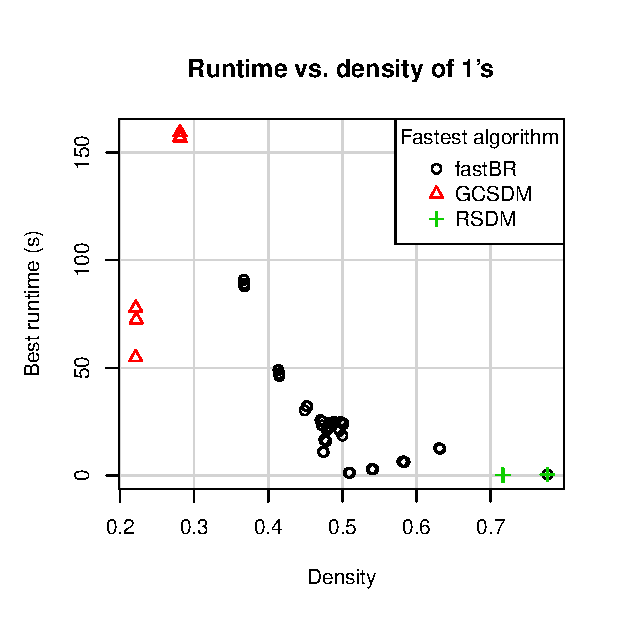
\includegraphics[height=8cm]{scatter_density.eps}
%		\end{center}
%		\caption{Fastest algorithm runtime vs. density of 1's for all $SBDMs$ under study.}
%		\label{fig:scattDensity}
%	\end{figure}	
%
%	Figure~\ref{fig:scattDensity} shows a scatter graph of the runtime as a function of 
%	the density of 1's in the $SBDM$. The runtime is taken from the fastest algorithm for 
%	each case. The dots are grouped by the best performing (fastest) algorithm for that particular 
%	matrix as shown in the legend of the figure. There can be identified three distinct groups of 
%	matrices by their density:
%	\begin{itemize}
%	\item Low density matrices: density $<$ 0.3.
%	\item Medium density matrices: 0.3 $<$ density $<$ 0.7.
%	\item High density matrices: density $>$ 0.7.
%	\end{itemize}
%	The fastest algorithm for low density matrices is GCSBDM, fastBR was the fastest for medium, and the three algorithms presented a similar performance for high	density matrices. The fact that high density $SBDMs$ do not constitute a complex computational task for reduct computation \citep{Rojas12} is clearly visible in Figure~\ref{fig:scattDensity}. 
%
%%	\begin{figure}[htb]
%%	    \begin{center}
%%	       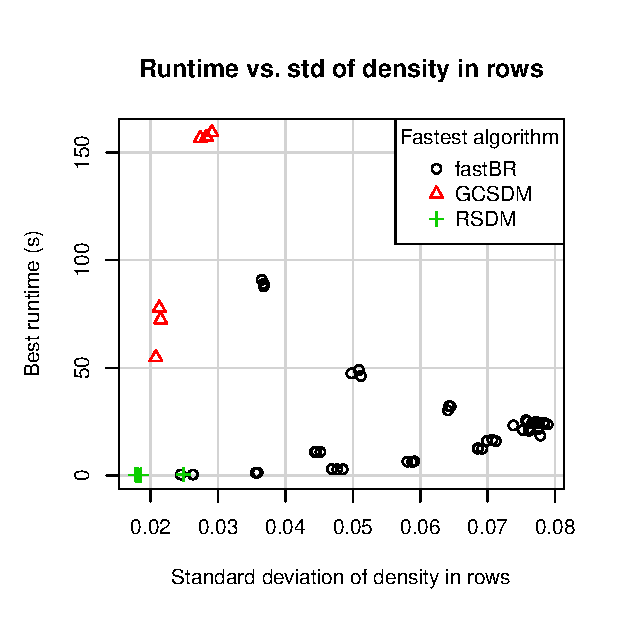
\includegraphics[height=8cm]{scatter_std.eps}
%%	    \end{center}
%%	\caption{Fastest algorithm runtime vs. standard deviation of density in rows for 
%%			 all $SBDMs$ under study.}
%%	\label{fig:scattStd}
%%	\end{figure}	
%	
%	Since all matrices for this experiment have the same dimensions, we can say that low density
%	matrices showed a relatively high complexity. For this reason, the apparent fact that GCSBDM outperforms 
%	the other algorithms for this kind of matrices, deserves special attention. 
%	
%	Figure~\ref{fig:scattStd} shows a scatter graph of the runtime as a function of 
%	the standard deviation of the density of 1's in the rows of the $SBDM$. As it can be seen, there is no
%	clear relationship between the runtime of the fastest algorithm and the standard deviation of density.
%	Notice (combining information from Figures~\ref{fig:scattDensity} and~\ref{fig:scattStd}) that both, 
%	low and high density matrices are related to low values of the standard deviation. In fact, it is not 
%	possible to increase the standard deviation in the extreme values of density.
%	
%	Figure~\ref{fig:TimeReducts} shows a scatter graph of the runtime as a function of the 
%	number of reducts in the $SBDM$. There can be seen a positive correlation between these two variables.
%	This is a natural trend, since the time complexity is at least as high as the space 
%	complexity; which exceeds the size of the solution. For high density matrices, there are a low number
%	of reducts which partially explains their lower computational cost (see Figure~\ref{fig:TimeReducts}). 
%	
%	\begin{figure}[htb]
%	    \begin{center}
%	       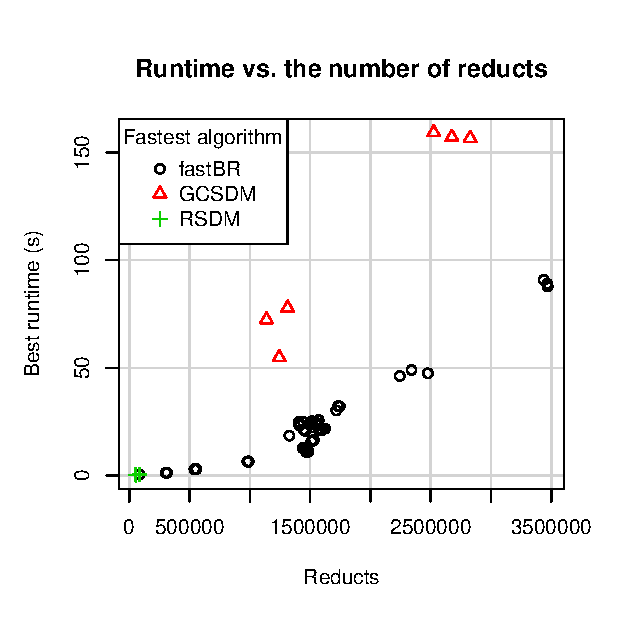
\includegraphics[height=8cm]{runtimeReducts.eps}
%	    \end{center}
%	\caption{Fastest algorithm runtime vs. the number of reducts.}
%	\label{fig:TimeReducts}
%	\end{figure}
%	\begin{figure}[htb]
%	    \begin{center}
%	       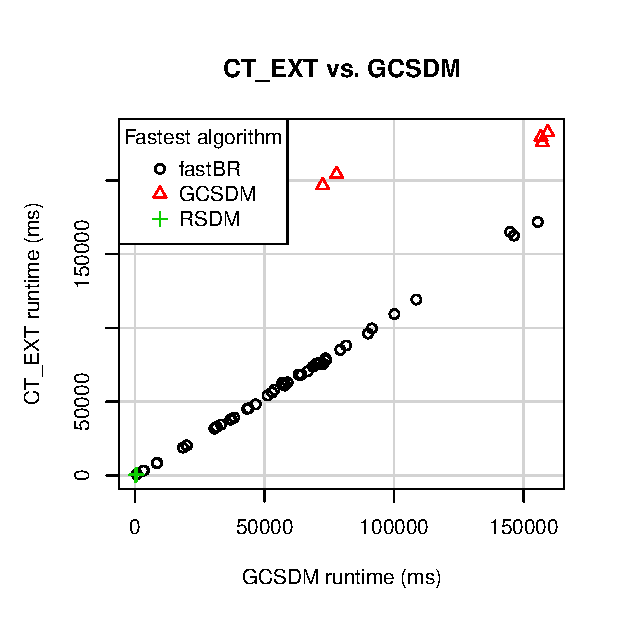
\includegraphics[height=8cm]{scatter_CTvsGAP.eps}
%	    \end{center}
%	\caption{CT\_EXT runtime vs. GCSBDM runtime.}
%	\label{fig:CTvsGAP}
%	\end{figure}		
%	
%	Figure~\ref{fig:CTvsGAP} shows a scatter graph of the runtime of CT\_EXT vs. GCSBDM for the $SBDMs$ used in
%	this experiment. Although GCSBDM outperforms CT\_EXT in most cases. Based on the evidence of
%	Figure~\ref{fig:CTvsGAP}, we proposed a one-sided t-test to evaluate the overall performance of GCSBDM over
%	CT\_EXT. Our \textbf{null hypothesis} is: \emph{there is no difference between the GCSBDM and CT\_EXT runtime}.
%	As \textbf{alternative hypothesis} we have: \emph{the runtime of CT\_EXT is higher than the runtime of GCSBDM}.
%	The output from the R software (Figure~\ref{fig:R_GCSBDM}) supports the alternative hypothesis beyond a 95\%
%	confidence interval. 
%	
%	\begin{figure}
%		\qquad{}	Paired one-sided t-test\\
%
%		data:  CT\_EXT runtime and GCSBDM runtime\\
%		t = 3.3, df = 56, p-value = 0.0008428\\
%		alternative hypothesis: true difference in means is greater than 0\\
%		95 percent confidence interval:\\
%		 6976.147ms  \qquad{}  Inf\\
%		sample estimates:\\
%		mean of the differences \\
%		 \qquad{}    14145.54ms
%		 
%		\centering
%	  	\caption{R output for the t-test of mean CT\_EXT and GCSBDM runtime.}
%	  	\label{fig:R_GCSBDM}
%	\end{figure}
%	
%	In order to evaluate the performance improvement of GCSBDM over fastBR, which is the fastest algorithm 
%	reported in the literature, we present a new experiment. A total 	of 83 low density matrices, with 30 
%	columns, was generated using the same procedure above described. This time, we generated $SBDMs$ with 1000 
%	rows. We evaluated the runtime of reduct computation over all matrices using fastBR and GCSBDM. 
%	Again we ran three execution of each possible combination in a randomized experiment.
%	
%	Figure~\ref{fig:runtime_low} shows the runtime as a function of the density of 1's in the $SBDM$.
%	There can be seen two interesting facts. First, there is a well defined
%	line delimiting those $SBDMs$ for which GCSBDM is faster than fastBR (densities under 0.3). Second, the
%	runtime of GCSBDM increases monotonically with the increase of the density of 1's in the $SBDM$.
%	
%	\begin{figure}[htb]
%	    \begin{center}
%	       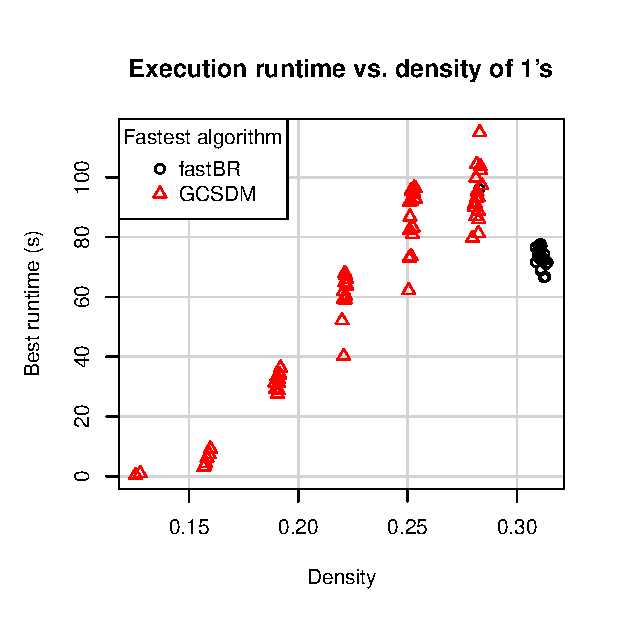
\includegraphics[height=8cm]{runtimeVSdensity_low.eps}
%	    \end{center}
%	\caption{Fastest algorithm runtime vs. density of 1's for all $SBDMs$ under study.}
%	\label{fig:runtime_low}
%	\end{figure}
%	\begin{figure}[htb]
%	    \begin{center}
%	       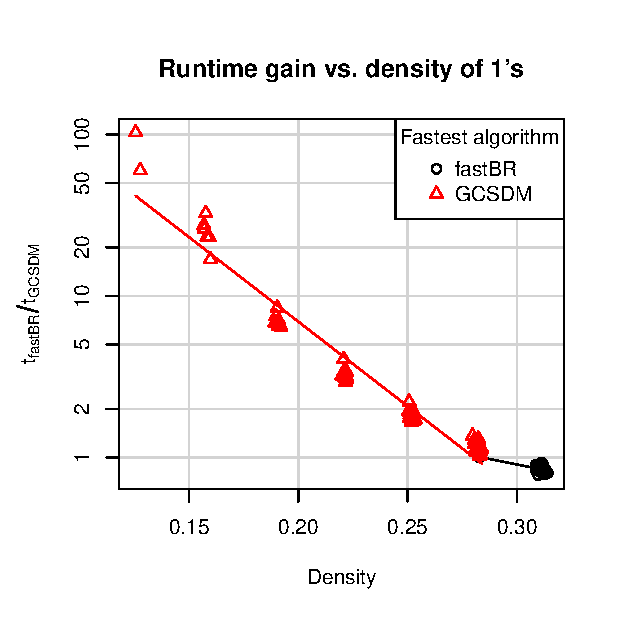
\includegraphics[height=8cm]{rate_runtime.eps}
%	    \end{center}
%	\caption{fastBR runtime over GCSBDM runtime  vs. density of 1's for all $SBDMs$ under study.}
%	\label{fig:BRvsGAP}	
%	\end{figure}	
%	
%	In Figure~\ref{fig:BRvsGAP} we show the runtime rate between fastBR and GCSBDM; where values above
%	1 mean a runtime improvement of GCSBDM over fastBR. For lower densities we have up to two orders of 
%	magnitude rate.
%	We found an exponential relationship between this rate and the density of the $SBDM$. Notice that the 
%	vertical axis in Figure~\ref{fig:BRvsGAP} is logarithmic.
%	
%	In order to explain this behaviour we must go deeply into the main difference between fastBR and GCSBDM. 
%	In GCSBDM we compute the exclusion mask and evaluate the proposition~\ref{prop:exclude} only for those
%	candidates proven as super-reducts, in order to verify them as reducts. In fastBR, on the other hand,
%	the proposition~\ref{prop:exclude} is evaluated for each contributing candidate. As a result, fastBR
%	evaluates less candidates than GCSBDM but at a higher cost per candidate. The attribute exclusion
%	occurs when there is at least one column, in the sub-matrix of $SBDM$ considering only the attributes in the 
%	current candidate, that can be removed without increasing the number of zero rows in this sub-matrix.
%	The exclusion is more frequent in matrices with a higher density of 1's, as it can be inferred from  
%	Figure~\ref{fig:BRvsGAP}. 
%	
%	Lets take for instance the extreme case of the identity matrix where there is no exclusion at all,
%	since every attribute is indispensable to form a reduct. 	For this $SBDM$, GCSBDM needs to evaluate as 
%	many candidates as fastBR but makes a single verification for exclusion with the set of all attributes. 
%	On the other hand, fastBR verifies the exclusion for each candidate, which leads to a higher 
%	computational cost.
%	
%	We used a one-sided t-test to evaluate the relative performance of GCSBDM over fastBR in
%	low density matrices. We selected the 62 $SBDMs$ having a density 	of 1's lower than 0.3, from our original 
%	83 matrices. As \textbf{null hypothesis} we have: \emph{there is no difference between the GCSBDM and fastBR 
%	runtime for $SBDMs$ with density of 1's lower than 0.3}. As \textbf{alternative hypothesis} we have: 
%	\emph{the runtime of fastBR is higher than the runtime of GCSBDM for $SBDMs$ with density of 1's lower than 
%	0.3}. The following output from the R software (Figure~\ref{fig:R_fastBRvsGCSBDM}) supports the alternative
%	hypothesis beyond a 95\% confidence interval.
%	
%	\begin{figure}
%		\qquad{}	Paired one-sided t-test\\
%
%		data:  fastBR runtime and GCSBDM runtime\\
%		t = 11.0838, df = 61, p-value $<$ 2.2e-16\\
%		alternative hypothesis: true difference in means is greater than 0\\
%		95 percent confidence interval:\\
%		 75124.33ms  \qquad{}  Inf\\
%		sample estimates:\\
%		mean of the differences \\
%		 \qquad{}    88453.32ms
%		 		 
%		\centering
%	  	\caption{R output for the t-test of mean fastBR and GCSBDM runtime.}
%	  	\label{fig:R_fastBRvsGCSBDM}
%	\end{figure}
	
%\newpage 
\section{Conclusions}\label{conclusions}
%	This PhD research proposal is focused on the problem of computing all the reducts and its related problem of
%	computing shortest reducts of an information system. These are problems with exponential complexity which are
%	actively studied. The theoretical bases were introduced to provide a unique nomenclature for the document and
%	ensure that it is self contained. We present a revision of the related work to show the most relevant 
%	approaches to the problem solution and based on this review we highlight the need for further research in this
%	area. Then, the PhD research proposal is introduced; including justification and motivation, research 
%	questions, our research objectives, and the methodology that will guide our research.
%	
%	As preliminary results, we we developed a hardware module for eliminating all non typical testors on the
%	hardware component; reducing the amount of data that must be transferred to the PC and eliminating the final
%	filtering. This hardware module is applicable to any algorithm for computing typical testors implemented on
%	FPGA devices. This result was published in the memories of an international conference on reconfigurable
%	computing.
%	Our second preliminary result is a new hardware architecture of the CT EXT algorithm (which is one of the 
%	most recent and fastest algorithms reported in the literature) for computing all the typical testors. Our 
%	proposal traverses the search space in a different order than previous works, which evaluates less candidate 
%	subsets than previous architectures, resulting in shorter runtime. This result has been reported in the 
%	journal of Expert Systems With Applications. Additionally, we proposed two new algorithms for computing all 	
%	the reducts, which are faster than existing algorithms for some kinds of datasets.
%	RSBDM was the fastest algorithm for $SBDMs$ with density above 0.7 while GCSBDM outperforms the rest of the
%	evaluated algorithms in $SBDMs$ with density under 0.3. These results will be reported in a congress or a 
%	journal specialized in Rough Set Theory.
%
%	Throughout our preliminary work, we covered most of the first four points in our proposed methodology, related
%	to algorithms for computing all reducts of an information system.
%	Finally, based on our preliminary results, we conclude that our objectives are reachable, in the scheduled
%	time, following 	the proposed methodology.
	
%-------------------------------------------------------------------------------
% Bibliography
%-------------------------------------------------------------------------------
\newpage 
\bibliography{mybib}{}
\bibliographystyle{authordate1}
\end{document}
